\documentclass{article}[10pt]
\usepackage[utf8]{inputenc}
\usepackage{tikz}
\usepackage{color}
\usepackage{subfiles}
\usepackage[T1]{fontenc}
\usepackage{titlepic}
\usepackage{amssymb}

\usepackage{graphicx}
\usepackage{caption}
\usepackage{subcaption}
\usepackage{amsmath}
\usepackage{algorithm2e}
\usepackage{algorithmic}
\usepackage{forest}

\usetikzlibrary{arrows,positioning, calc}
\tikzstyle{vertex}=[draw,fill=black!15,circle,minimum size=18pt,inner sep=0pt]

\tikzset{
  treenode/.style = {align=center, inner sep=0pt, text centered,
    font=\sffamily},
  arn_n/.style = {treenode, circle, white, font=\sffamily\bfseries, draw=black,
    fill=black, text width=1.5em},% arbre rouge noir, noeud noir
  arn_r/.style = {treenode, circle, red, draw=red, 
    text width=1.5em, very thick},% arbre rouge noir, noeud rouge
  arn_x/.style = {treenode, rectangle, draw=black,
    minimum width=0.5em, minimum height=0.5em}% arbre rouge noir, nil
}


\title{\Huge{Red Black Tree} \\\Large{A Balanced Binary Tree} }
\author{S.M. Kausar Parvej \\
        \textbf{Id: 2005076} 
        \and 
        Sagor Chanda \\
        \textbf{Id: 2005071}
        \and 
        Souvik Mandal \\
        \textbf{Id: 2005069}}
\date{\today}


\begin{document}

\maketitle

\vspace{4cm}

\begin{figure}[h!]
\centering
    
\includegraphics[width = 0.25\textwidth]{Pictures/logoBUET.png}
\end{figure}
\begin{center}

\vspace{.5cm}

\Large{Department of Computer Science and Engineering \\
    Bangladesh University of Engineering and Technology \\ }

\end{center}

\newpage

\tableofcontents
\newpage

% \listoffigures
% \newpage

\section{Introduction}
Trees are well-known as a non-linear data structure\cite{weiss2007data}. They don’t store data in a linear way. They organize data hierarchically. One specific type of a tree is Binary Search Tree. The binary search tree data structure supports many dynamic-set operations, including
SEARCH, MINIMUM, MAXIMUM, PREDECESSOR, SUCCESSOR, INSERTION, and DELETION.\\

\label{sec:intro}

\begin{figure}[h]
    \centering
    \subfile{Pictures/BST1.tex}
    \caption{Example of a Tree}
    \label{fig:Tree}
\end{figure}


But these basic operations on a binary search tree take time proportional to the height of the tree. For a complete binary tree with n nodes, such operations run in $\mathcal{O}(\log n)$ worst-case time. If the tree is a linear chain of n nodes, however, the same operations take $\mathcal{O}(n)$ worst-case time. So we need trees which can balance it's height by itself. Red Black Tree is a kind of such Height Balanced Binary Search Trees.


\section{Red Black Tree}
A red–black tree is a kind of self-balancing binary search tree in computer science. Each node of the binary tree has an extra bit, and that bit is often interpreted as the color (red or black) of the node. 
By constraining the node colors on any simple path from the root to a leaf, red-black trees ensure that no such path is more than twice as long as any other. 
The tree is thus approximately height balanced.
Each node of the tree now contains the attributes
\textit{color, key, left, right, and p.} If
a child or the parent of a node does not exist, the corresponding pointer attribute of the node contains the value \texttt{NIL}. These \texttt{NILs} are regarded as being pointers to leaves (external nodes) of the binary search tree and the normal, key-bearing nodes as being internal nodes of the tree.


\section{Properties}

            The properties\cite{introAlgo} of a Red Black Tree is given below:
            \begin{enumerate}
                
                \item \textcolor{red}{Color Property:} Each node is either red or black.
                \item \textcolor{red}{Root Property:} The root is black
                \item \textcolor{red}{External Property:} Every external node is black
                \item \textcolor{red}{Internal Property:} Both children of a red node are black.
                \item \textcolor{red}{Depth Property:} For each node, all simple paths from the node to descendant leaves contain the same number of black nodes.
            \end{enumerate}

        
       \begin{figure}[h]
            
           \centering
            \subfile{Pictures/RBTP1.tex}
           \caption{Properties of a Red Black Tree}
           \label{fig:Properties of RBT}
       \end{figure}
    
The number of black nodes from the root to a node is the node's black depth; the uniform number of black nodes in all paths from root to the leaves is called the black-height of the red–black tree.

These constraints enforce a critical property of red–black trees: the path from the root to the farthest leaf is no more than twice as long as the path from the root to the nearest leaf. The result is that the tree is roughly height-balanced. Since operations such as inserting, deleting, and finding values require worst-case time proportional to the height of the tree, this theoretical upper bound on the height allows red–black trees to be efficient in the worst case, unlike ordinary binary search trees.

To see why this is guaranteed, it suffices to consider the effect of properties 4 and 5 together. For a red–black tree T, let B be the number of black nodes in property 5. Let the shortest possible path from the root of T to any leaf consist of B black nodes. Longer possible paths may be constructed by inserting red nodes. However, property 4 makes it impossible to insert more than one consecutive red node. Therefore, ignoring any black NIL leaves, the longest possible path consists of $2 \times B$ nodes, alternating black and red (this is the worst case). Counting the black NIL leaves, the longest possible path consists of $2 \times B - 1$ nodes.

The shortest possible path has all black nodes, and the longest possible path alternates between red and black nodes. Since all maximal paths have the same number of black nodes, by property 5, this shows that no path is more than twice as long as any other path.

\section{How Red Black Tree is Height Balanced}

Red Black Tree for storing n items will have a height of $\mathcal{O}(n)$\cite{sedgewick2011algorithms}. So, it will remain height balanced.

    \begin{enumerate}
        \item the subtree rooted at any node x contains at least $2^{bh(x)} - 1$  internal nodes. 
        \item If $h(x) = 0$ then $x$ is a leaf, so the subtree rooted at x contains $2^0-1 = 0$ internal nodes.
        \item For a node x with positive height and two children, the black height of the children will be $ bh(x) $ (for red internal node) or  $bh(x) - 1$ (for black internal node).
        
        
    \end{enumerate}
    \begin{center}
        \subfile{Pictures/RBTThm1.tex}
        \vspace{1cm}
        \subfile{Pictures/RBTThm2.tex}
        \vspace{1cm}
        \subfile{Pictures/RBTThm3.tex}
            
    \end{center}
   
    
    
    
 So, using induction, we can prove subtree rooted at x contains at least 
 \begin{itemize}
     \item $(2^{bh(x)-1}-1) + (2^{bh(x)-1}-1) + 1 = (2^{bh(x)} -1)$ internal nodes.
    \item According to the internal property the black-height of the root must be at least $\frac{h}{2}$; thus
    \item  $n \geqslant 2^{\frac{h}{2}}-1$
	\item  $\log(n+1) \geqslant \frac{h}{2}$
	\item $h \geqslant 2\log(n+1)$	
	\item Thus $h = \mathcal{O}(\log(n))$
    \end{itemize}        


\section{Operations}
As discussed in Section \ref{sec:intro}, Red Black Trees can perform dynamic-set operations like other binary search trees. But the main advantage with Red Black Trees is they have balanced height and so those operations can be done in $\mathcal{O}(\log n)$ time in every case.

\subsection{Searching}
Searching in a Red Black Tree is not different than any other Binary Search Tree. We start searching from the root and compare every node with our desired key. While searching, if the required key is greater than the key of the node we are comparing with, we will go to the right child, and if it is less we will go to the left child, and repeat the same. If we reach a leaf node in this way, we can decide that the key is not in there in the tree.\\ 
The algorithm to search\cite{introAlgo} a key in a binary tree is given below. Here we will start from the root of the tree. Input x is initially root and input k is the desired key.\\

\subfile{Operations/RBTSearch.tex}

An example of searching 22 is simulated below in Figures \ref{fig:search1} to \ref{fig:search4}:\\

\begin{figure}[htbp]
	\centering
	\subfile{Pictures/RBTS1.tex}
	\caption{Seaching 22 : Step 1} 
	\label{fig:search1}
\end{figure}

\begin{figure}
	\centering
	\subfile{Pictures/RBTS2.tex}
	\caption{Seaching 22 : Step 2} 
	\label{fig:search2}
\end{figure}

\begin{figure}
	\centering
	\subfile{Pictures/RBTS3.tex}
	\caption{Seaching 22 : Step 3}
	\label{fig:search3}
\end{figure}

\begin{figure}
	\centering
	\subfile{Pictures/RBTS4.tex}
	\caption{Seaching 22 : Step 4} % subcaption
	\label{fig:search4}
\end{figure}


\newpage
\subsection{Insertion}
Insertion begins by adding the node in a very similar manner as a standard binary search tree insertion and by coloring it red. The big difference is that in the binary search tree a new node is added as a leaf, whereas leaves contain no information in the red–black tree, so instead the new node replaces an existing leaf and then has two black leaves of its own added. \\
What happens next depends on the color of other nearby nodes. There are several cases of red–black tree insertion to handle:
\begin{enumerate}
    \item New Node (\textbf{N}) is the root node, i.e., first node of red–black tree
    \item \textbf{N}'s parent (\textbf{P}) is black
    \item \textbf{P} is red (so it can't be the root of the tree) and N's uncle (\textbf{U}) is red
    \item \textbf{P} is red and \textbf{U} is black
\end{enumerate}

\begin{description}
    \item[\textbf{Case 1:}]    
                The current node \textbf{N} is at the root of the tree. In this case, it is repainted black to satisfy property 2 (the root is black). Since this adds one black node to every path at once, property 5 (all paths from any given node to its leaf nodes contain the same number of black nodes) is not violated.
    \item[\textbf{Case 2:}]    
                The current node's parent \textbf{P} is black, so property 4 (both children of every red node are black) is not invalidated. In this case, the tree is still valid. Property 5 (all paths from any given node to its leaf nodes contain the same number of black nodes) is not threatened, because the current node N has two black leaf children, but because \textbf{N} is red, the paths through each of its children have the same number of black nodes as the path through the leaf it replaced, which was black, and so this property remains satisfied.   
    \item[\textbf{Case 3:}]    
                If both the parent \textbf{P} and the uncle \textbf{U} are red, then both of them can be repainted black and the grandparent \textbf{G} becomes red to maintain property 5 (all paths from any given node to its leaf nodes contain the same number of black nodes). Since any path through the parent or uncle must pass through the grandparent, the number of black nodes on these paths has not changed. However, the grandparent \textbf{G} may now violate Property 2 (The root is black) if it is the root or Property 4 (Both children of every red node are black) if it has a red parent. To fix this, the tree's red-black repair procedure is rerun on G.\\Note that this is a tail-recursive call, so it could be rewritten as a loop. Since this is the only loop, and any rotations occur after this loop, this proves that a constant number of rotations occur.
    \item[\textbf{Case 4, step 1:}]    
                The parent \textbf{P} is red but the uncle \textbf{U} is black. The ultimate goal will be to rotate the current node into the grandparent position, but this will not work if the current node is on the "inside" of the subtree under \textbf{G} (i.e., if \textbf{N} is the left child of the right child of the grandparent or the right child of the left child of the grandparent). In this case, a left rotation on \textbf{P} that switches the roles of the current node \textbf{N} and its parent \textbf{P} can be performed. The rotation causes some paths (those in the sub-tree labeled "1") to pass through the node \textbf{N} where they did not before. It also causes some paths (those in the sub-tree labeled "3") not to pass through the node P where they did before. However, both of these nodes are red, so property 5 (all paths from any given node to its leaf nodes contain the same number of black nodes) is not violated by the rotation. After this step has been completed, property 4 (both children of every red node are black) is still violated, but now we can resolve this by continuing to step 2.
    \item[\textbf{Case 4, step 2:}]    
                The current node \textbf{N} is now certain to be on the "outside" of the subtree under \textbf{G} (left of left child or right of right child). In this case, a right rotation on \textbf{G} is performed; the result is a tree where the former parent \textbf{P} is now the parent of both the current node N and the former grandparent \textbf{G}. G is known to be black, since its former child \textbf{P} could not have been red without violating property 4. Once the colors of \textbf{P} and \textbf{G} are switched, the resulting tree satisfies property 4 (both children of every red node are black). Property 5 (all paths from any given node to its leaf nodes contain the same number of black nodes) also remains satisfied, since all paths that went through any of these three nodes went through \textbf{G} before, and now they all go through \textbf{P}.
\end{description}
In the algorithm\cite{introAlgo} above, all cases are called only once, except in Case 3 where it can recurse back to Case 1 with the grandparent node, which is the only case where an iterative implementation will effectively loop. Because the problem of repair in that case is escalated two levels higher each time, it takes maximally $\frac{h}{2}$ iterations to repair the tree (where h is the height of the tree). Because the probability for escalation decreases exponentially with each iteration the average insertion cost is practically constant.\\
All these cases can be handles in the algorithm\cite{introAlgo} stated below:
\\
\subfile{Operations/RBTInsert.tex}
\vspace{0.5cm}
and the RB\_Insert\_Fixup is: \\
\subfile{Operations/RBTInsertFixup.tex}
\vspace{0.5cm}
%%%ALGORITHM FILES%%%

To construct a Red Black Tree consecutive insertions are performed. An example of inserting keys ${2,3,5,7,4}$ consecutively into an initially empty tree is given below in Figures \ref{fig:insert1} to \ref{fig:insert5}:

\begin{figure}[htbp]
	\centering
	\subfile{Pictures/RBTI1.tex}
	\caption{Inserting 2} 
	\label{fig:insert1}
\end{figure}

\begin{figure}
	\centering
	\subfile{Pictures/RBTI2.tex}
	\caption{Inserting 3}
	\label{fig:insert2}
\end{figure}

\begin{figure}
	\centering
	\subfile{Pictures/RBTI3.tex}
	\caption{Inserting 5} 
	\label{fig:insert3}
\end{figure}

\begin{figure}
	\centering
	\subfile{Pictures/RBTI4.tex}
	\caption{Inserting 7} 
	\label{fig:insert4}
\end{figure}

\begin{figure}
	\centering
	\subfile{Pictures/RBTI5.tex}
	\caption{Inserting 4}
	\label{fig:insert5}
\end{figure}


%%%%%%%%%%%%%%%%%






\subsection{Deletion}
Like the other basic operations on an n-node red-black tree, deletion of a node takes
time $\mathcal{O}(n)$. Deleting a node from a red-black tree is a bit more complicated than inserting a node. \\
In order to simplify boundary conditions in the code, we use a sentinel to represent \textbf{NIL}. For a red-black tree T, the sentinel \textit{nil[T]} is an object with the same fields as an ordinary node in the tree. Its color field is BLACK, and its other fields--p, left, right, and key--can be set to arbitrary values. In the red-black tree, all pointers to \textbf{NIL} are replaced by pointers to the sentinel \textit{nil[T]}.

We use sentinels so that we can treat a \textbf{NIL} child of a node x as an ordinary node whose parent is x. We could add a distinct sentinel node for each \textbf{NIL} in the tree, so that the parent of each \textbf{NIL} is well defined, but that would waste space. Instead, we use the one sentinel nil[T] to represent all the \textbf{NIL'S}. When we wish to manipulate a child of a node \textit{x}, however, we must be careful to set \textit{p[nil[T]]} to \textit{x} first.

The procedure RB-DELETE\cite{introAlgo} is a minor modification of the TREE-DELETE procedure. After splicing out a node, it calls an auxiliary procedure \textbf{RB-DELETE-FIXUP} that changes colors and performs rotations to restore the red-black properties. \\
\\
\subfile{Operations/RBTDelete.tex}
\vspace{0.5cm}
We can now examine how the procedure RB-DELETE-FIXUP restores the red-black properties to the search tree. \\
\\
\subfile{Operations/RBTDeleteFixup.tex}
\vspace{0.5cm}
There are several cases of red–black tree deletion to handle: \\
\begin{description}
        \item[\textbf{Case 1:}]    
                This occurs when node \textit{w}, the sibling of node \textit{x}, is red. Since \textit{w} must have black children, we can switch the colors of \textit{w} and \textit{p[x]} and then perform a left-rotation on \textit{p[x]} without violating any of the red-black properties. The new sibling of \textit{x}, one of \textit{w}'s children, is now black, and thus we have converted case 1 into case 2, 3, or 4.
        \item[\textbf{Case 2:}]    
                In case 2 both of \textit{w}'s children are black. Since \textit{w} is also black, we take one black off both \textit{x} and \textit{w}, leaving \textit{x} with only one black and leaving \textit{w} red, and add an extra black to \textit{p[x]}. We then repeat the while loop with \textit{p[x]} as the new node \textit{x}. Observe that if we enter case 2 through case 1, the color \textit{c} of the new node \textit{x} is red, since the original \textit{p[x]} was red, and thus the loop terminates when it tests the loop condition.\\
        \item[\textbf{Case 3:}]    
                This case occurs when \textit{w} is black, its left child is red, and its right child is black. We can switch the colors of \textit{w} and its left child \textit{left[w]} and then perform a right rotation on w without violating any of the red-black properties. The new sibling \textit{w} of \textit{x} is now a black node with a red right child, and thus we have transformed case 3 into case 4.
        \item[\textbf{Case 4:}]    
                This case occurs when node \textit{x}'s sibling w is black and \textit{w}'s right child is red. By making some color changes and performing a left rotation on \textit{p[x]}, we can remove the extra black on \textit{x} without violating any of the red-black properties. Setting \textit{x} to be the root causes the while loop to terminate when it tests the loop condition.
\begin{figure}[h]
    \centering
    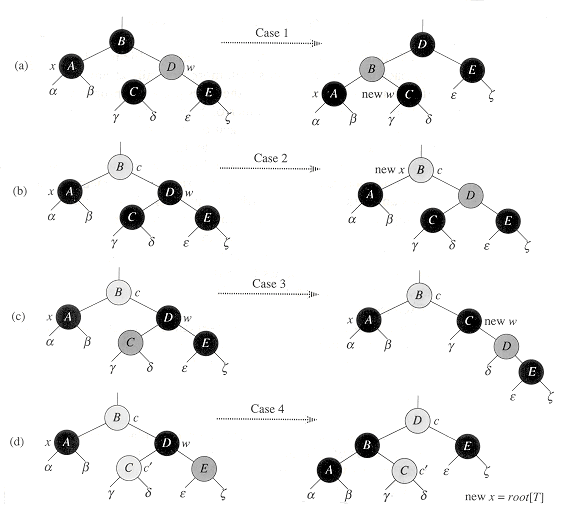
\includegraphics[scale=0.6]{Pictures/Del.png}
    \caption{Red-Black Tree Deletion}
\end{figure}
\end{description}




\section{Practical Applications}
Red-black trees have numerous practical applications\cite{goodrich2013data} across various domains due to their efficient balancing properties and optimized operations. Let's drive into some detailed practical applications of red-black trees: 

\begin{itemize}
    \item Red-Black Trees are crucial for organizing files efficiently in file systems. 
    \item Red-Black Trees enable quick retrieval of records in databases based on keys. 
    \item Red-Black Trees are used to implement symbol tables for quick lookup of
    identifiers in compilers.  
\end{itemize}


\section{Conclusion}

Balanced search trees have a height that is always $\mathcal{O}(\log n)$. One consequence of this is that lookup, insert, and delete on a balanced search tree can be done in $\mathcal{O}(\log n)$ worst-case time. In constrast, binary search trees have a worst-case height of $\mathcal{O}(n)$ and lookup, insert, and delete are $\mathcal{O}(n)$ in the worst-case. Red-black trees are just one example of a balanced search tree.

Red-black trees are binary search trees that store one additional piece of information in each node (the node's color) and satisfy three properties\cite{weiss2007data} These properties deal with the way nodes can be colored (the root property and the red property) and the number of black nodes along paths from the root node to a null child pointer (the black property). Although it is not intuitively obvious, the algorithms for restoring these properties after a node has been added or removed result in a tree that stays balanced.\\
Red-black trees offer efficient insertion, deletion and lookup operations, all with a worst-case time complexity of $\mathcal{O}(n)$. This is a significant improvement over binary search trees, where these operations can degrade to $\mathcal{O}(n)$ in the worst case. The algorithms for insertion and deletion in red-black trees ensure that the tree maintains its balance while satisfying the properties of red-black trees. During insertion, if the properties are violated, the tree is re-balanced through rotations and recoloring operations, ensuring that the height of the tree remains logarithmic. Similarly, deletion operations are carefully managed to maintain the balance and properties of the tree. As a result, red-black trees provide consistent and efficient performance for dynamic data structures, making them suitable for a wide range of applications.

Lookup operations in red-black trees are also optimized for efficiency. The properties of red-black trees guarantee that the path from the root to any leaf has at most twice as many black nodes as any other path, ensuring balanced access times for all elements in the tree. This balanced access pattern, combined with the logarithmic height of the tree, ensures that lookup operations are fast and predictable, even in the worst-case scenarios.

Red-black trees are not only important theoretically but also have significant practical implications in computer science. Their efficient balancing properties make them ideal for various applications where dynamic sets or maps are required. For instance, they are widely used in the implementation of associative arrays, symbol tables, and in the internals of many popular data structures and algorithms, such as Java's\cite{weiss2007data} Tree-Map and Tree-Set.\\
Moreover, the $\mathcal{O}(\log n)$ worst-case time complexity of operations like lookup, insert, and delete ensures predictable performance, making red-black trees suitable for real-time systems and applications where performance is critical. Additionally, their self-balancing nature reduces the chances of worst-case scenarios, providing a reliable and consistent performance guarantee even in dynamic environments.

Furthermore, red-black trees serve as a foundational concept in understanding more advanced balanced search trees and algorithms. Knowledge of their properties and operations provides a solid basis for exploring more complex data structures and algorithms, such as AVL trees, B-trees, and various self-adjusting binary search trees.

In conclusion, the study and understanding of red-black trees not only contribute to the development of efficient data structures and algorithms but also play a vital role in enhancing the performance and reliability of software systems across various domains.



\bibliographystyle{abbrv}
\bibliography{ref}
\end{document}